\documentclass[a4paper,12pt]{article}
\usepackage[utf8]{inputenc}
\usepackage{color}
\usepackage{graphicx}
\usepackage{amsmath}

\begin{document}


\title{CSE 376: Technical Writing and Presentation\\Homework - Latex Checkpoints}
\author{Asif Idris Tuhin }
\date{\today}

\maketitle

\pagenumbering{roman}

\tableofcontents
\newpage
\pagenumbering{arabic}


\section{Checkpoint 1}
\label{checkpoint1}

\subsection{experimenteing1}
Experimenting 1st subsection
\subsection{experimenteing2}
Experimenting 2nd subsection
\subsection{experimenteing3}
Experimenting 3rd subsection
\subsection{Label Checking}
Referring to \ref{checkpoint1} No. section on page \pageref{checkpoint1}

\newpage
\section{Checkpoint 2}

\subsection{Font Effects}
\textit{Technical Writing and Presentation}\\
\textbf{Technical Writing and Presentation}\\
\textsl{Technical Writing and Presentation}\\
\textsc{Technical Writing and Presentation}\\
\texttt{Technical Writing and Presentation}\\
\textsf{Technical Writing and Presentation}\\
\textrm{Technical Writing and Presentation}\\
\underline{Technical Writing and Presentation}

\subsection{coloured Text}
{\color{green}Technical Writing and Presentation}\\
{\color{red}fire}

\subsection{Font Sizes}
{\tiny tiny HELLO WORLD}
{\scriptsize scriptsize Hello World}
{\footnotesize footnotesize Hello World}
{\small small Hello World}\\
{\normalsize normalsize Hello World}\\
{\large large Hello World}\\
{\Large Large Hello World}\\
{\huge huge Hello World}\\
{\LARGE LARGE Hello World}\\
{\Huge Huge Hello World }

\subsection{Lists}
\begin{enumerate}
\item 1st paper
\item 2nd paper
\begin{itemize}
\item one category
\item two category
\item[@] without bullet category
\end{itemize}
\item 3rd paper
\end{enumerate}

\subsection{Comment and Spacing}
It is very interesting learing %latex , i will keep trying.
Everyone should try this.\\
New line but not new paragraph

Hello         World with new paragraph and new line.

\vspace{50pt}
This line is vertically spaced by 50pt

\subsection{Special Characters}
\#
\$ 
\% 
\^{} 
\& 
\_ 
\{
\}
\~{}
\textbackslash

\vspace{12pt}
/

\vspace{70pt}
Item \#1A\textbackslash642 costs \$8 \& is sold at a \~{}10\% profit.

\vspace{50pt}
%\newpage
\section{Checkpoint 3}

\subsection{1st table}
\begin{table}[h]
    \centering
    \begin{tabular}{l|r|r}
    Item    &   Quantity   &    Price (\$)\\
    \hline
    Nails   &   500    &    0.34   \\
    Wooden Boards   &   100    &    4.00   \\
    Bricks  &   240    &    11.50   \\

    \end{tabular}

\end{table}

\newpage

\subsection{2nd table}
\begin{table}[h]
    \centering
    \begin{tabular}{l|ccc}
        &  \multicolumn{3}{|c}{Year} \\
        \cline{2-4}
        City &  2006    &   2007    &   2008\\
        \hline
        London  & 45789 & 46551 & 51298 \\
        Berlin  & 34549 & 32543 & 29870 \\
        Paris   & 49835 & 51009 & 51970 \\
    \end{tabular}    
\end{table}

\section{Checkpoint 4}
\begin{figure}[h!]
    \centering
    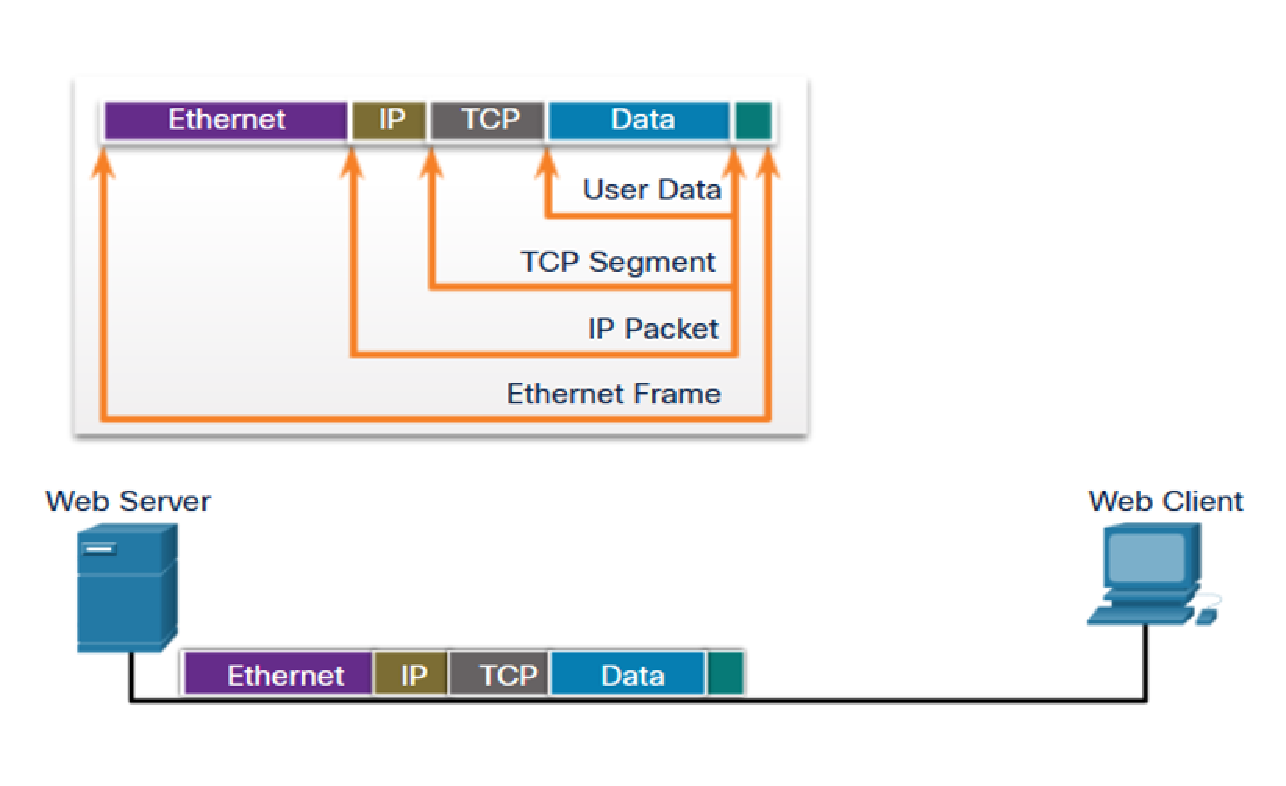
\includegraphics[width=1\textwidth]{networkingCapture.pdf}
    \caption{My test Image}
    \label{fig:network}
\end{figure}

{\Large Shown in figure \ref{fig:network} on page no. \pageref{fig:network}}

\newpage

\section{Checkpoint 5}
\begin{equation}
    e=mc^2
\end{equation}

\begin{equation}
    \pi=\frac{c}{d}
\end{equation}

\begin{equation}
    \frac{d}{dx}e^x=e^x
\end{equation}

\begin{equation}
    \frac{d}{d x}\int_{0}^{\infty} f(s)ds=f(x)
\end{equation}

\begin{equation}
    f(x)=\sum_{i}=0^{\infty}\frac{f^{(i)}(0)}{i!}x^{i}
\end{equation}

\begin{equation}
    x=\sqrt{\frac{x_i}{z}y}
\end{equation}

\begin{equation}
    \left[
    \begin{matrix}
    1 & 2 & 3 & 4 & 5 \\
    6 & 7 & 8 & 9 & 10 \\
    11 & 12 & 13 & 14 & 15 \\
    16 & 17 & 18 & 19 & 20 \\
    21 & 22 & 23 & 24 & 25
    \end{matrix}
    \right]
\end{equation}


\newpage

\section{Checkpoint 6}
Let's create some references!!!
this is references no \cite{wohn2011s}
this is references no \cite{ducheneaut2006alone}
this is references no \cite{freeman2015simulating}
this is references no \cite{freeman2016intimate}
this is references no \cite{freeman2016revisiting}
this is references no \cite{hamari2017esports}
this is references no \cite{hamilton2012high}
\cite{hamilton2012pen}
\cite{jonasson2010electronic}
\cite{kaytoue2012watch}
\cite{kostakos2005social}
\cite{kow2013media}
\cite{leavitt2016ping}
\cite{lee2011comparison}
\cite{wagner1968glaser}


\bibliographystyle{plain}
\bibliography{references}
\end{document}
